\documentclass[border=10pt]{standalone}

\usepackage{tikz}
\usepackage{tikzsymbols}
\usetikzlibrary{calc,patterns,shapes.geometric}

\def\centerarc[#1](#2)(#3:#4:#5){\draw[#1] ($(#2)+({#5*cos(#3)},{#5*sin(#3)})$) arc (#3:#4:#5);}

\begin{document}
	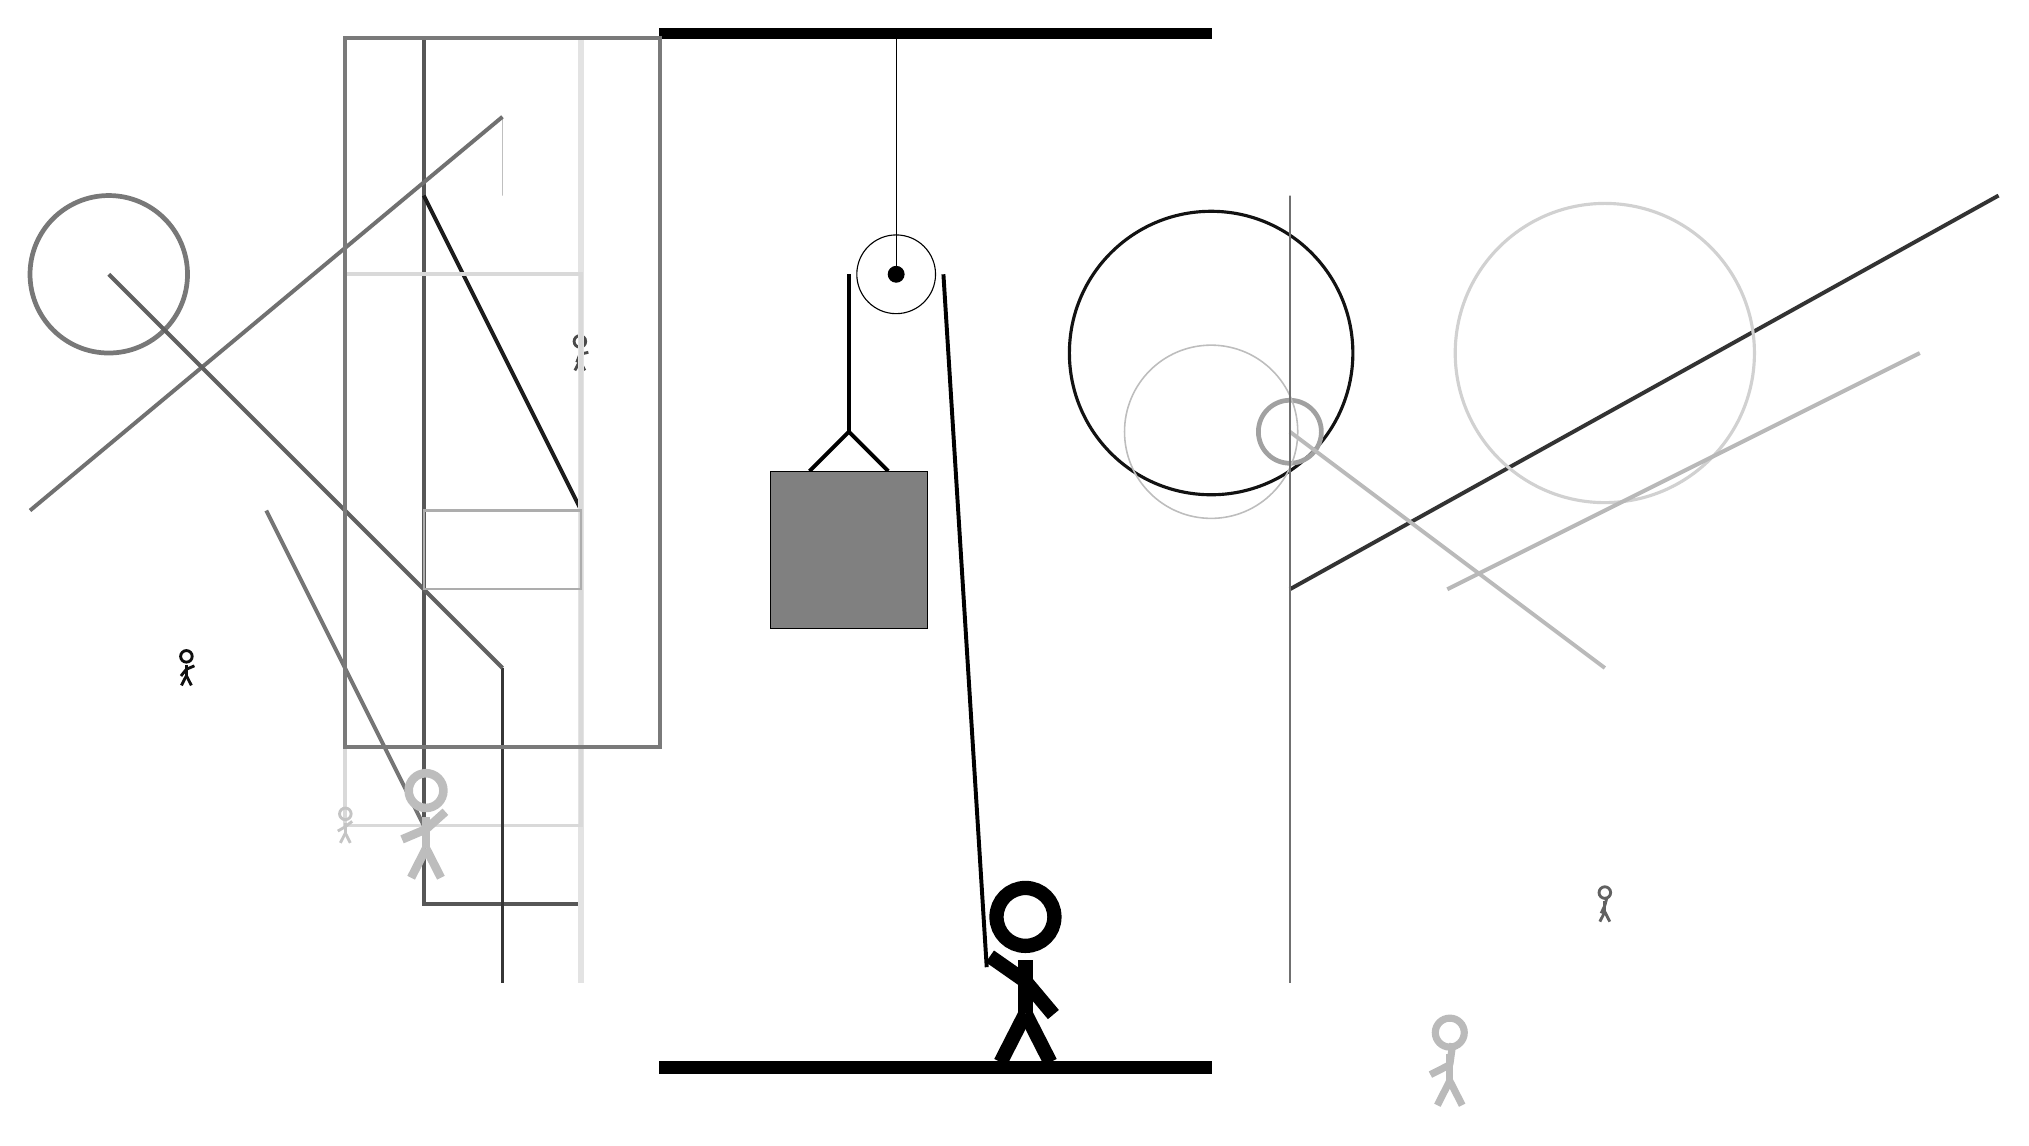
\begin{tikzpicture}
		%%%%% START %%%%%
		
		\draw[fill=black] (-2, 10) rectangle (5, 10.125);
		
		\draw (1, 7) circle (0.5);
		\draw[fill=black] (1, 7) circle (0.1);
		\draw (1, 10) -- (1, 7);
		
		\draw[line width=0.5mm, color=black!66] (-3, 10) rectangle (-5, -1);
		
		\draw[line width=0.2mm, color=black!25] (-4, 8) rectangle (-4, 9);
		\draw[line width=0.5mm, color=black!80](6, 3) -- (15, 8);
		\draw [line width=0.6mm, color=black!53](-9, 7) circle (1.0);
		\draw[line width=0.5mm, color=black!89](-3, 4) -- (-5, 8);
		\node[line width=0.6mm, color=black!71] at (-3, 6) {\Strichmaxerl[2][69][13]};
		\draw[line width=0.7mm, color=black!11] (-3, -2) rectangle (-3, 10);
		
		\draw [line width=0.4mm, color=black!93](5, 6) circle (1.8);
		\draw [line width=0.6mm, color=black!37](6, 5) circle (0.4);
		
		\draw[line width=0.5mm, color=black!15] (-3, 7) rectangle (-6, 0);
		\draw[line width=0.5mm, color=black!27](10, 2) -- (6, 5);
		
		\draw[line width=0.5mm, color=black!56](-4, 9) -- (-10, 4);
		\draw[line width=0.5mm, color=black!79] (-4, 2) rectangle (-4, -2);
		\draw [line width=0.2mm, color=black!26](5, 5) circle (1.1);
		\draw[line width=0.5mm, color=black!54](-5, 0) -- (-7, 4);
		\node[line width=0.5mm, color=black!62] at (10, -1) {\Strichmaxerl[2][65][75]};
		
		\draw[line width=0.2mm, color=black!56] (6, -2) rectangle (6, 8);
		\node[line width=0.5mm, color=black!23] at (-6, 0) {\Strichmaxerl[2][30][38]};
		\node[line width=0.5mm, color=black!27] at (8, -3) {\Strichmaxerl[5][27][82]};
		\draw[line width=0.5mm, color=black!62](-4, 2) -- (-9, 7);
		\node[line width=0.4mm, color=black!26] at (-5, 0) {\Strichmaxerl[6][23][42]};
		\draw[line width=0.5mm, color=black!52] (-2, 10) rectangle (-6, 1);
		\draw[line width=0.3mm, color=black!32] (-3, 4) rectangle (-5, 3);
		\draw [line width=0.4mm, color=black!18](10, 6) circle (1.9);
		\node[line width=0.6mm, color=black!94] at (-8, 2) {\Strichmaxerl[2][51][23]};
		
		\draw[line width=0.5mm, color=black!28](8, 3) -- (14, 6);
		
		\draw[line width=0.5mm] (-0.1, 4.5) -- (0.4, 5.0) -- (0.9, 4.5);
		\draw[fill=black!50] (-0.6, 4.5) rectangle (1.4, 2.5);
		
		\draw[line width=0.5mm] (0.4, 7) -- (0.4, 5.0);
		\centerarc[line width=0.5mm](1, 7)(0:180:0.6);
		\draw[line width=0.5mm](1.6, 7) -- (2.15, -1.8);
		
		\node at (2.6, -1.9) {\Strichmaxerl[10][-35][-50]};
		
		\draw[fill=black] (-2, -3) rectangle (5, -3.15);
		
		%%%%% END %%%%%
	\end{tikzpicture}
\end{document}